% ---------------------------------------------------------------------------
% Author guideline and sample document for EG publication using LaTeX2e input
% D.Fellner, v1.11, Feb 28, 2005

\documentclass{egpubl}

% --- for  Annual CONFERENCE
% \ConferenceSubmission % uncomment for Conference submission
 \ConferencePaper      % uncomment for (final) Conference Paper
% \STAR                 % uncomment for STAR contribution
% \Tutorial             % uncomment for Tutorial contribution
% \ShortPresentation    % uncomment for (final) Short Conference Presentation
%
% --- for  CGF Journal
% \JournalSubmission    % uncomment for submission to Computer Graphics Forum
% \JournalPaper         % uncomment for final version of Journal Paper
%
% --- for  EG Workshop Proceedings
% \WsSubmission    % uncomment for submission to EG Workshop
% \WsPaper         % uncomment for final version of EG Workshop contribution
%
 \electronicVersion % uncomment if producing the printed version

% for including postscript figures
% mind: package option 'draft' will replace PS figure by a filename within a frame
\ifpdf \usepackage[pdftex]{graphicx} \pdfcompresslevel=9
\else \usepackage[dvips]{graphicx} \fi

\PrintedOrElectronic

% prepare for electronic version of your document
\usepackage{t1enc,dfadobe}

\usepackage{egweblnk}
\usepackage{cite}
\usepackage{verbatim} 
\usepackage{subfigure}

% For backwards compatibility to old LaTeX type font selection.
% Uncomment if your document adheres to LaTeX2e recommendations.
\let\rm=\rmfamily    \let\sf=\sffamily    \let\tt=\ttfamily
\let\it=\itshape     \let\sl=\slshape     \let\sc=\scshape
\let\bf=\bfseries

% end of prologue





% ---------------------------------------------------------------------
% EG author guidelines plus sample file for EG publication using LaTeX2e input
% D.Fellner, v1.12, Oct 21, 2005

\title[Designing a Sketch Recognition Front-End: User Perception of
Interface Elements]
      {Designing a Sketch Recognition Front-End: User Perception of
Interface Elements}
%\title[Iterative Design of a Sketch-Based Tool for Pedagogical Circuit Design]%
%      {Iterative Design of a Sketch-Based Tool for Pedagogical Circuit Design}

% for anonymous conference submission please enter your SUBMISSION ID
% instead of the author's name (and leave the affiliation blank) !!
\author[P. Wais, C. Alvarado, and A. Wolin]
       {P. Wais$^1$, C. Alvarado$^1$, and A. Wolin$^1$
%        S. Spencer$^2$\thanks{Chairman Siggraph Publications Board}
        \\
         $^1$Department of Computer Science, Harvey Mudd College, Claremont, CA\\
%        $^2$ Another Department to illustrate the use in papers from authors
%             with different affiliations
       }

% ------------------------------------------------------------------------

% if the Editors-in-Chief have given you the data, you may uncomment
% the following five lines and insert it here
%
% \volume{23}   % the volume in which the issue will be published;
% \issue{2}     % the issue number of the publication
% \pStartPage{201}      % set starting page


%-------------------------------------------------------------------------
\begin{document}

\maketitle

\begin{abstract}
   Programs that can recognize students' hand-drawn diagrams have the
   potential to revolutionize education by breaking down the barriers
   between diagram creation and simulation.  Much recent work focuses
   on building robust recognition engines, but understanding how to
   support this new interaction paradigm from a user's perspective is
   an equally important, and less well understood, problem.  We
   present a user study that investigates four critical sketch
   recognition user interface issues: how users integrate the process
   of triggering recognition into their work, when users prefer to
   indicate which portions of the diagram should be recognized, how
   users prefer to receive recognition feedback, and how users
   perceive recognition errors.  We find that user preferences
   emphasize the importance of system reliability, the minimization of
   distractions, and the maximization of predictability. 
   
% Contribution: This paper presents the first direct comparison of critical
%  free-sketch recognition user interface mechanisms through the novel
%  application of a Wizard of Oz evaluation methodology.  We present
%  recommendation for developers of sketch recognition user interfaces 
%  as well as an interface for a sketch recognition digital design tool 
%  informed by our results.


% Benefit: The results of our study directly inform key aspects of
%   sketch recognition user interface design (e.g., how to allow users
%   to trigger recognition and how to provide recognition feedback),
%   and recognition algorithm development (e.g., which types of errors
%   to try to avoid). 

% Research areas:
%  Evaluation
%  Pen UIs
%  Recognition of sketches, diagrams... etc.

% For additional keywords I would list:
% Wizard of Oz Study

 

% results:
% users want reliability of button trigger over convenience of gesture
% users want pre-separation over post separation and want seperation tool to require least work
% users want most efficient interface possible
% users want least invasive feedback; feedback that provides most natural transformation
% users want most predictible errors
% users all use more or less the same approach to using our tool


%%% QUESTION %%%
% which or how many of these classifications make sense?
% also, do we put email next to ByLine?

\begin{classification} % according to http://www.acm.org/class/1998/
\CCScat{H.5.2}{User Interfaces}:\textit{Evaluation/methodology, Interaction styles, Prototyping, User-centered design}
\end{classification}

\begin{classification} % according to http://www.acm.org/class/1998/
\CCScat{I.5.4}{Computing Methodologies}{Pattern Recognition}{Applications}
\end{classification}

%\begin{classification} % according to http://www.acm.org/class/1998/
%\CCScat{J.6}{Computer-Aided Engineering}{Computer-aided design}
%\end{classification}

%\begin{classification} % according to http://www.acm.org/class/1998/
%\CCScat{I.3.3}{Computer Graphics}{Line and Curve Generation}
%\end{classification}

%\begin{classification} % according to http://www.acm.org/class/1998/
%\CCScat{H.1.2}{User/Machine Systems}{Human information processing}
%\end{classification}

\end{abstract}


%-------------------------------------------------------------------------
\section{Introduction}

% example of frustration: += thomas "adapt correct behavior to work for it" is a problem
% intro += crossY CrossY \cite{1029635}

The field of pedagogical sketch-based systems is currently a thriving
area of research.  Many engineering classes rely on
simulation technologies to help students understand the systems they
design.  Unfortunately, mouse and keyboard interfaces to these
programs are cumbersome, and many students commit considerable time
and effort to learning how to use and troubleshoot simulation
software.  Furthermore, though coursework relies heavily on this
software, students nevertheless draw countless diagrams on paper (or
on the Tablet PC) while completing homework and laboratory problems
because paper is a faster and more natural way to quickly create a
diagram.  In fact, many instructors require students to draw their
diagrams on paper before entering them into simulation software so
that they focus on their design, not on the software interface.
Elimination or simplification of the process of transforming circuit
diagrams to code through the utilization of pedagogical sketch-based
systems allows for a novel learning process and reduces the
implementation effort that this process requires of the student.

% Not sure about this sentence.
%Furthermore, circuit
%diagrams created in the design process are primary communication
%artifacts.  
% Paul's comment: my point was to emphasize the importance of diagrams in
% student communication... I think this sentence is a result of the influences
% of my anthropology professor if anything :)

Several existing systems demonstrate the success of integrating sketch
understanding into pedagogical software for numerous domains,
including physics and math\cite{LaViola2006Initial},
chemistry\cite{Tenneson2005ChemPad}, and electrical
engineering\cite{KaraStahovich04SimuSketch}, but these systems face
their own interface challenges.

%  Furthermore, much progress has been made
%in the development of sketch recognition algorithms\cite{LaViola2006Initial} and
%several systems have exhibited successful applications of hybrid
%classification systems\cite{1029636} and probabilistic
%frameworks\cite{Alvarado2004SketchRead}[WeeSan's 06 or WeeSan's 07].  Most
%importantly, users demonstrate a clear desire for sketch understanding
%in our own investigation.
% 
% Might be possible to integrate this text into the above paragraph.


The first challenge is the question of how to allow users to trigger
recognition and how to display recognition feedback.  Feedback can be
distracting in the early stages of design \cite{Hong2002Sketch}, but
it can also aid recognition as it can help the user adapt their
drawing style to match the system's expectations.  Researchers have
evaluated the usability of various recognition triggers and feedback
mecahnisms in isolation (e.g.,
\cite{Alvarado2001Preserving,Newman2003Denim,LaViola2006Initial}), but
have not compared different techniques directly.

A second challenge is to determine how to allow the user to indicate
which pieces of the diagram the system should attempt to recognize.
Students' homework often consists of a mix of text, equations, and
diagrams. Despite advances in parsing heterogeneous
notes~\cite{Wang2006Parsing}, a recognition system must receive only a
single type of input to be practical.  Most recognition systems allow
the user to draw only one type of input (e.g., electrical
circuits~\cite{Gennari2005Combining}), while other systems allow the
user to manually select pieces of their drawing to be recognized after
they have finished drawing~\cite{LaViola2006Initial}.  Again, little
is known about which interface users prefer.


A third challenge is to minimize the impact of recognition errors on
usability.  Researchers are working to address this challenge in many
ways.  Some systems reduce errors by placing constraints on the users'
drawing style.  Matching these constraints to the way users draw
naturally can aid recognition without forcing the user to conform to
unnatural drawing styles~\cite{Alvarado2007Properties}.  Others have
focused on intuitive error correction mechanisms as a way of reducing
the impact of recognition errors~\cite{Mankoff2000Providing}.  Finally,
understanding users' tolerance for different types of recognition
errors can help guide sketch recognition research by allowing
researchers to focus on eliminating errors that have the biggest
impact on usability.  Little work has been done in this area.

%Richard Davis' SketchWizard (ref SketchWizard) takes the first stride towards constructing a generic, multi-domain tool for %conducting Wizard-of-Oz-based development of sketch-based systems.  Our technique entails the mobilization of SketchWizard's %Wizard of Oz paradigm while simultaneously engineering a Tablet PC application front-end that could potentially wrap future %sketch-recognition engines for further user studies.  


%  through the novel
%application of a Wizard of Oz evaluation methodology.  We present
%  an interface for a sketch recognition digital design tool 
%  informed by our results.
  
To address the above challenges, we present the first direct
comparison of critical free-sketch recognition user interface
elements.  Unlike prior research, which usually involves a qualitative
analysis of a complete solution, we compare interface elements
directly through a novel application of a Wizard of Oz evaluation
methodology.  Specifically, we evaluate UI mechanisms for triggering
recognition, providing feedback, separating recognized from
unrecognized data, and we examine users' perception of different types
of recognition errors including misrecognized symbols and incorrectly
grouped strokes.  Our study addresses the following questions:
\begin{itemize}
\item How do users integrate the task of triggering recognition into
their workflows?  How can the design of a user interface assist in
this integration?
\item How do users react to and interpret recognition results?  
\item How and when do users perfer to indicate which pieces of the
  diagram should be recognized? 
\item How do recognition errors effect the user experience? 
\item In the domain of digital circuit design, what characteristics of
a sketch-based system do users find most desirable?
\end{itemize}

Our results indicate that:
\begin{itemize}
\item Users prefer to trigger recognition after they are done drawing,
  even when the system produces errors
\item Users prefer to segregate pieces of the drawing (e.g., diagram
  vs. annotation) at creation time rather than recognition time
\item Users want recognition feedback to transform their strokes as
  little as possible (even though they are done sketching)
\item Users prefer errors that are predictable
\end{itemize}

One important user interface question that we do not address is how
gesture-based or menu-based interfaces compare to free-sketch
recognition interfaces.  For example, users might prefer a reliable
gesture-based system to an error-prone free-sketch recognition system.
Although this question is important, we focus only on free-sketch
recognition interfaces for two reasons.  First, the students we talked
to expressed a strong desire for a system that could simply transform
the drawings they already produce into recognized circuit schematics;
they did not want to have to learn a whole new language for
interacting with the simulation software.  Second, we cannot compare
free-sketch recognition systems to gesture or menu-based systems until
we better understand how to design an effective user interface for
these systems.

Our study was conducted in a single domain (digital circuit design)
and so directly informs the design of a sketch recognition interface
for digital circuit design.  However, we believe these preferences may
apply to other domains.  \emph{Need a stronger sentence here.}


%-------------------------------------------------------------------------
\section{Related Work}

%\textit{Long and scanscribe references in comments below:}
% Quill 2001 #1: http://citeseer.ist.psu.edu/485742.html
% Quill 2001 #2: http://portal.acm.org/citation.cfm?id=971510&dl=&coll=&CFID=15151515&CFTOKEN=6184618
% Scanscribe 2004 #1 & #2: http://www2.parc.com/isl/members/saund/papers.html

Previous user studies of sketch-based user interfaces have focused
mainly on the development or evaluation of complete systems.
Researchers rely heavily on interviews and ethnographic studies to
help them understand what users desire in a sketch-based computer
tool.  For example, Landay and Myers designed
SILK~\cite{landay95SILK}, a sketch-based system for user interface
design, based on the results of a survey of professional user
interface developers.  Newman \textit{et al.} worked closely with
desginers throughout the design of DENIM~\cite{Newman2003Denim}, a
sketch-based system for web page design.  Their interaction with users
revealed that web page development requires very little sketch
recognition: DENIM recognizes pages (rectangles) and links (arrows)
but leaves the rest of the user's sketch unrecognized.  DENIM relies
on recognizing gestures, rather than freely-drawn sketches, thus
avoiding many of the user interface issues we examine.  Other domains
require a deeper understanding of the user's sketch.  For example, in
order to simulate a student's circuit, the system must understand all
of the components in the circuit and how they are connected.

Evaluations of more recognition-intensive systems provide some insight
about how users prefer to interact with these systems.  Evaluation of
many recognition-intensive systems tends to focus on recognition error
rates, and provide only general insight into user interface issues
(e.g., ``users liked the system'' or ``users found recognition errors
frustrating'')~\cite{Alvarado2001Preserving,Gennari2005Combining,Hammond2002Tahuti}.
A few researchers, however, have examined system usability in more
detail.  LaViola's evaluation of MathPad$^{2}$, a sketch-based system
that recognizes freely-drawn equations and physical diagrams, reveals
specific user preferences such as the fact that users like the
scribble erase gesture, and they find recognition errors frustrating,
but tolerable for this task~\cite{LaViola2006Initial}.  Other studies
of recognition-based user interfaces are currently underway, but
results are still forthcoming
\cite{Koile2007Supporting,Tenneson2005ChemPad}.  Evaluating a complete
system, while important, does not allow researchers to directly
compare interface elements because of the difficulty in modifying the
system.  Our Wizard of Oz methogology allows us to simulate a complete
recognition system so that we can easily modify user interface
elements and determine user preferences for specific interface
elements rather than assess the suitability of a completed system for
its domain.


Other researchers have studied the usability of pen-based interaction
techniques that are complementary to sketch recognition.  The CrossY
interface~\cite{Apitz04CrossY} presents several novel interface
elements that combine gestures and WIMP components.  Long \textit{et
al.}~\cite{Long00VisualSimilarity} provide a model for measuring the
visual similarity of gestures and a system that helps users design
those gestures~\cite{Long2001Quill} in an effort to inform effective
gesture design.  Finally Lank and Saund present a model of users'
pen-based selection gestures to inform the design of a faster, more
accurate selection mechanism \cite{Lank2005Sloppy}.  The results of
these previous studies are complementary to our results in the
creation of a complete sketch recognition system.


%% Progress in the development of sketch recognition systems has focused
%% primarly the refinement of recognition algorithms and the devising of
%% recognition-supported interaction pardigms.
%% SimuSketch\cite{KaraStahovich04SimuSketch} and MathPad$^{2}$ support
%% interaction paradigms similar to that of our goal system.  Users of
%% SimuSkech and MathPad sketch diagrams, recognize sketches, and finally
%% conduct a simulation based upon the understood sketch.  The developers
%% of these systems support their target interaction paradigms with
%% intelligently chosen interface elements but do not investigate the
%% effectiveness of these interface elements in isolation.  SimuSketch
%% celebrates elimination of a cumbersome interface constraint that
%% requires users to indicate to the system when a complete symbol has
%% been drawn.  Furthemore, Kara and Stahovich explicate issues
%% surrounding the approach of triggerig recognition on demand versus
%% triggering recognition automatically after each stroke but they do not
%% evaluate these two interaction techniques head-to-head.  MathPad
%% relies heavily on gesture-based triggers and requires a considerably
%% lengthy training process to calibrate recognition.
%% (SketchRead~\cite{Alvarado2004SketchRead} requires no trainining and
%% presents few constraints on user sketches but presents no evaluation
%% of this interaction technique.  Irrelvant point?)

Finally, though little is known about how free sketch recognition
errors affect usability, researchers have studied user perception of
handwriting and speech recognition errors.  Rhyne and Wolf present
early work in this area, laying out important considerations for the
design of recognition-based user
interfaces~\cite{Rhyne1993Recognition}.  More recently, Frankish
\textit{et al.} find that error rates directly impact user acceptance
of systems; furthermore, the relationship between error rates and user
acceptance is dependent on the perceived cost to benefit ratio of a
specific task~\cite{Frankish95RecogAccuracy}.  We expect that the same
trend holds for sketch recognition systems.  Wu \textit{et al.} found
that handwriting task completion time is most sensative to error rates
above 6\%, thus there is a point of deminishing returns in the pursuit
of the minimization of error rates ~\cite{Wu03ChineseCharacterRecog}.
Munteanu \textit{et al.} find a linear relationship between speech
recognition accuracy and user experience with webcasts.  While we do
not examine error rates specifically, our analysis helps inform user
perception of sketch recognition errors.

\section{User interface elements}

Our goal was to evaluate UI mechanisms for triggering recognition, providing
feedback, separating recognized from unrecognized data, and we examine
users' perception of different types of recognition errors including
misrecognized symbols.  The reactions of participants in our pre-study
verified that users are indeed sensitive to the interface elements
that support the sketch recognition interaction paradigm.  This
section describes the specific mechanisms we compared for each of
these points.


%\subsection{Recognition Triggers}
We compared three different methods for triggering recognition present
in existing applications or suggested by participants in our pre-study:
button, gesture and pause.  

\begin{itemize}
\item \textbf{Button Trigger}  The user triggers
recognition by tapping on a large interface button.  Many sketch
recognition interfaces use this trigger.
\item \textbf{Gesture Trigger}  The user triggers
recognition using a ``check-tap'' gesture (a
check mark followed by a tap).  We
selected this gesture because in informal tests it seemed to be
reliably recognized, not easily confused with with sketching strokes,
and similar to (but simpler than) the ``circle-tap'' gesture used in
MathPad$^2$.  
\item \textbf{Automatic Trigger: Pause Trigger.}  The system triggers
recognition automatically after a brief pause (4 seconds) in
sketching.  Serveral pre-study participants indicated that they would
like to use this recognition trigger.
\end{itemize}

%%   We conjectured that system-triggered
%% recognition may entice users to engage in a ``dialog'' with the system
%% (e.g., users will treat the system like an agent).  Furthermore, users
%% might find that system-triggered recognition maximizes sketching
%% efficiency. \emph{Say something about no cognitive overhead for
%%   recognition--it just happens.  Paul's note: see \LaTeX\ comment below 
%%   for pre-study link if that's helpful. }
%% We conjecture that users might find gesture-based
%% triggers more convenient, efficient, and natural.

% Pre-study notes are at: https://www.cs.hmc.edu/twiki/bin/view/Sketchers/UserTestingNotes


%% \begin{figure}[tb]
%%   \centering
%%   
\includegraphics{checkTapDemo.png}
%%   \caption{\label{fig:checkTapDemo}
%%            fig G = Check-Tap Gesture.}
%% \end{figure}

\begin{figure}[tb]
  \centering
  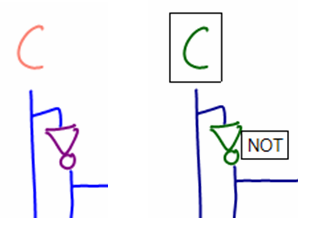
\includegraphics[width=.75\linewidth]{feedbackDemo.png}
  \caption{\label{fig:feedbackDemo}
           Text and color feedback comparison.}
\end{figure}

%\subsection{Specifying Strokes to Recognize}

The second issue we explored was how to allow the user to indicate
which strokes the system should recognize.  Students' drawing
generally consist of diagrams, notes and annotations.  Manually
separating notes from diagrams reduces the complexity of the sketches
that a recognition engine must parse.  Sometimes it is feasible to
provide separate note and diagrams panels, but when users want to make
annotations directly on the diagram, this setup is not feasible.  We
examined two techniques for allowing users to segregate annoatations
(unrecognized) from diagrams (recognized).

\begin{itemize}
\item \textbf{Pre-separation: ``Color'' Tool} This version of the
  interface requires users to separate domain-relevant strokes from
  annotation-relevant strokes sa they draw by toggling between stylus
  modes using a button.  The system uses ink color to indicate the
  current mode: in sketch mode, the stylus draws black ink; in
  annotation mode, the stylus draws gray ink (hence we call this
  option the ``color tool'').
\item \textbf{Post-separation: Lasso Tool} The user draws sketches and
  annotations freely, but then must lasso-select strokes to be
  recognized (similar to the interaction mechanism in
  MathPad$^{2}$\cite{1015741}).  The user executes a check-tap gesture
  to switch to lasso-selection mode, lassos the portion of the sketch
  she wants recognized, and check-taps again to trigger recognition.  
\end{itemize}

%\subsection{Feedback Mechanisms}
The third issue we explored is how provide the user with recognition
feedback.  We compared two different methods, based on techniques
used by other recognition systems and pre-study interviews: color feedback, 
and text labels (Figure~\ref{fig:feedbackDemo}).  We rejected the idea of
replacing the user's strokes with symbols based on lack of common
interest in this idea during pre-studies and the results of previous
work~\cite{Hong2002Sketch}.

\begin{itemize}
\item \textbf{Color Feedback} The system displays each recognized
symbol in a unique color.  In addition, users can see a text label by
hovering over the strokes in the symbol.  
\item \textbf{Text-Label Feedback.}  The system draws text labels next
to recognized symbols.
\end{itemize}


%% \textit{I took out these sentences because I'm not sure we want to
%%   hypothesize here.}
%% Color: We conjecture that this
%% feedback mechanism might prove the easiest to interpret and the most
%% comfortable to visually recognize.  

%% Text: We conjecture that this
%% feedback mechanism might prove the easiest to interpret and the most
%% comfortable to visually recognize.  



%\subsection{Impact of Recognition Error}
Finally, we examined how errors impact the user experience.
Recognition errors are a primary source of user frustration with
sketch recognition systems.  Understanding how users perceive errors
enables system designers to tailor their user interfaces and their
recognition algorithms to cope with and avoid particularly frustrating
errors.

%Furthermore, the visibility of
%recognition errors is inherently confounded with the effectiveness
%feedback mechanisms.  

We investigate how three types of common recognition errors impact the
user experience: false positives, false negatives and stroke grouping
errors (Figure \ref{fig:errorDemo}).  False positives occur when the
system incorrectly identifies a symbol (e.g., labels an AND gate as an
OR gate); false negatives (or \textit{omissions}) occur when the
system fails to identify a symbol; and grouping errors occur when the
system incorrectly adds or removes adjacent strokes to or from a
symbol.


\begin{figure}[tb]
  \centering
  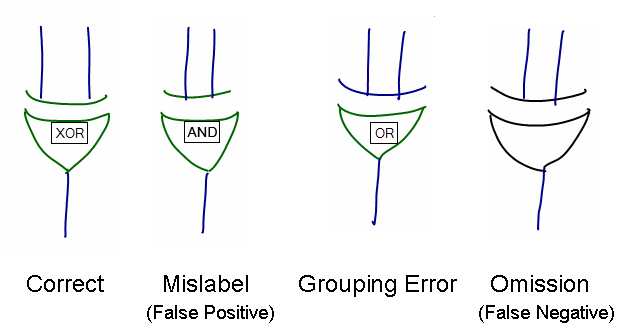
\includegraphics{errorDemo.png}
  \caption{\label{fig:errorDemo}
           Illustration of different error types}
\end{figure}

%-------------------------------------------------------------------------
\section{Experimental Design}
For this study, we limit our scope to digital circuit design in order
to keep tasks consistent across all users in order to better
understand how interface decisions (as opposed to domain variability)
affect usability.  While focusing on a single domain limits the
generality of our results somewhat, the style of the design task we
explored is representative of educational design tasks in many fields.

\subsection{Tasks and Participants}
Users in our study designed circuits based on truth table function
representations---a common task in an introductory digital design
class.  Figure~\ref{fig:tt-task} gives an example of one of these
tasks.  Given the truth table, the user must determine how to combine
the inputs using logic gates to produce the correct outputs
(Figure~\ref{fig:tt-solution} shows one possible circuit for the task in
Figure~\ref{fig:tt-task}).  Users were allowed to use any method to
create the circuit, and they were not required to simplify their
circuit (although they could if they wanted to).  In some cases
(described in the next section) we also asked uses to annotate the
shortest and longest path through the circuit they designed.



 \begin{figure}[tb]
 \centering
 \begin{tabular}{p{.85\linewidth}}
 	Please draw a circuit diagram for the following truth table:
 	\end{tabular}

   \subfigure[Truth table task] {
   	\label{fig:tt-task}

 			
      \begin{tabular}{|l|l|l||l|l|}
      \hline 
      \multicolumn{3}{|c||}{Input} & \multicolumn{2}{c|}{Output} \\
      \hline
      A & B & C & F & G \\
      \hline
      0 & 0 & 0 & 0 & 1 \\
      \hline
      0 & 0 & 1 & 0 & 0 \\
      \hline
      0 & 1 & 0 & 0 & 1 \\
      \hline
      0 & 1 & 1 & 0 & 0 \\
      \hline
      1 & 0 & 0 & 0 & 0 \\
      \hline
      1 & 0 & 1 & 0 & 0 \\
      \hline
      1 & 1 & 0 & 1 & 0 \\
      \hline  
      1 & 1 & 1 & 1 & 1 \\
      \hline        
    \end{tabular}
} 
%		\vspace{3pt}

		%% \begin{tabular}{p{.85\linewidth}}
%% 		Please notify the experimenter when you are satisfied with the design of your circuit and you can confirm that the system has correctly recognized all of your strokes.\\
%% 		\end{tabular}\\

   \subfigure[A possible solution (with color feedback).  The black dot
     denotes the user's stylus] {
     	\label{fig:tt-solution}
 	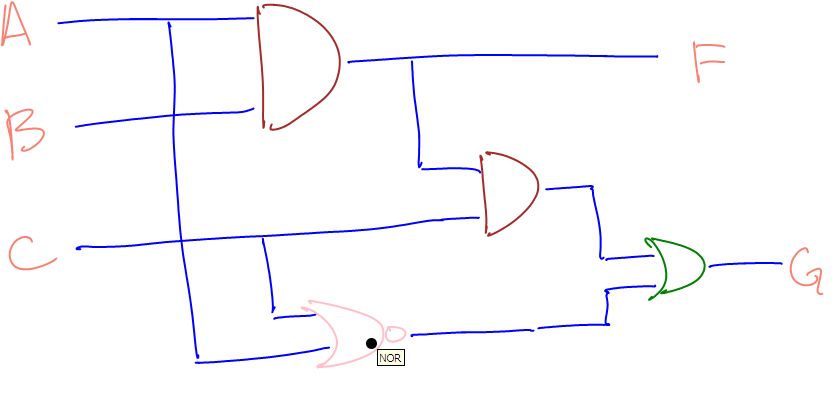
\includegraphics[width=1.0\linewidth]{complete.png}  
   }
	
 	\caption{ A truth table task from our user study}
 \end{figure}


%\begin{figure*}[tb]
%  \centering
%  \subfigure[Truth table task]{
%  	\label{fig:tt-task}
%    \textit{Given the truth table below, sketch the corresponding schematic}
%    \begin{tabular}[|l|l|l|l]
%      \hline 
%      \multicolumn{3}{l}{Input} & Output \\
%      \hline
%     0 & 0 & 0 & 0 \\
%     \hline
%     0 & 0 & 1 & 1 \\
%     \hline
%      0 & 1 & 0 & 0 \\
%      \hline
%      0 & 1 & 1 & 0 \\
%      \hline
%     1 & 0 & 0 & 1 \\
%      \hline      
%    \end{tabular}
%    \label{fig:tt-task}
%  }
%  \subfigure[Possible solution]{
%%    \includegraphics[width=0.5\linewidth]{Figures/instr_060130_slide11}
%    %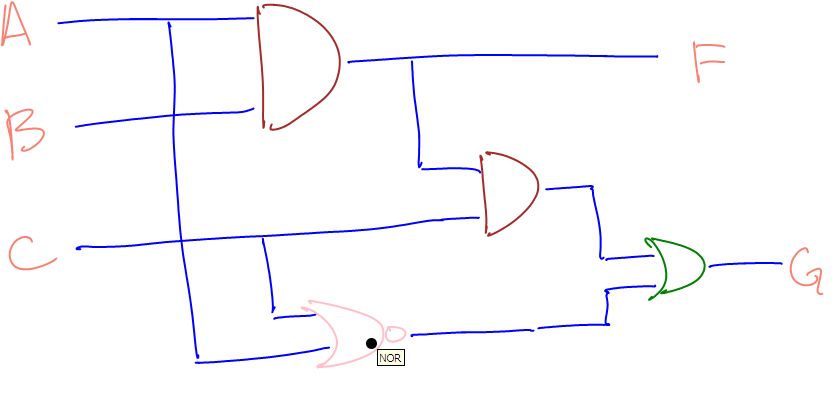
\includegraphics[width=\linewidth]{complete.png}
%    \label{fig:tt-result}
%  }
%  \caption{A task from our user study}
%  \label{fig:task}
%\end{figure*}


In a pre-study we determined that these tasks are relatively short yet
non-trivial, requiring the mental energy of a typical homework
problem.  We also verified that all of our tasks were uniformly
difficult by asking six pre-study participants to rate the difficulty
of several tasks and selecting only those tasks that users rated as
similarly difficult.  These small circuit design tasks require enough
mental concentration that most of our participants needed to write
notes to support their design processes. 

Users completed a fixed set of circuit design tasks.  For each task we
varied one aspect of the user interface.  We describe the details of
each of the user interface elements we varied below.  Each participant
completed between three and five tasks, and each session lasted 45-60
minutes.

In total, nine people (six male and three female) participated in our
formal tests (not including the pre-studies). All participants were
Claremont College students who had taken an introductory digital
circuit design class.  All participants had used digital circuit
simulation software (Xilinx) in their coursework.  Six of these
students had previous experience (more than an hour) with a Tablet PC,
and five had taken notes on a Tablet PC during their digital design
course (without recognition, using Windows Journal or One Note).

\subsection{Basic Interface Design}
Our goal was to compare various user interface elements for a sketch
recognition system that supports the task of digital circuit
design. To examine this issue, we first had to design a prototype
interface and determine which specific interface elements to compare.

\begin{figure}[tb]
  \centering
  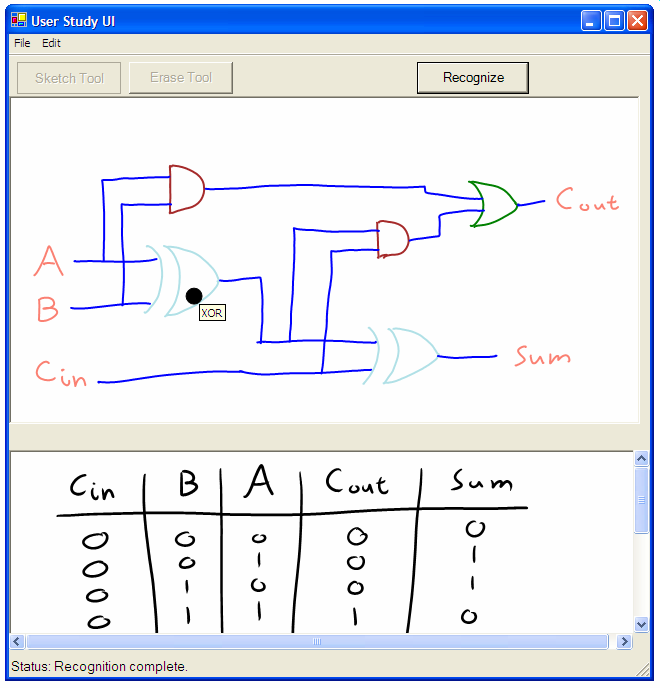
\includegraphics[width=1.0\linewidth]{fullGUIdemo.png}
  \label{fig:fullGUIdemo}
  \caption{
           Complete sketch recognition interface }
\end{figure}

We designed our basic interface using interative design techniques.
Through interviews and informal studies with paper prototypes we
identified a common interaction paradigm across users: a user draws
notes or equations, sketches a circuit schematic, triggers recognition
of the schematic, and finally corrects any recognition errors before
loading the understood circuit into a simulation program.
Figure~\ref{fig:fullGUIdemo} shows a basic overview of our final
interface, although we modified pieces of this interface to explore
different interface elements (which we describe below).  In the
displayed version of the interface, the user sketches notes (unrecognized)
in the bottom panel, sketches the circuit in the top panel
(recognized) and presses the ``Recognize'' button to trigger
recognition.  

Users could correct recognition errors only by erasing and redrawing
their strokes.  We did not aim to explore error correction mechanisms,
and this method was adequate for users to complete their tasks, but we
discuss the potential implecations of this error correction method on
our results below.


%% Not needed--too much detail.  In general, only talk about what
%% you actually did, not what you planned to do.

%% Furthermore, the manual correction of errors can itself be a
%% frustrating process.  Participants of our paper prototype study
%% suggested several different correction mechanisms.  Potentially useful
%% correction mechanisms include:\\

%% \textbf{Correction Mechanisms} 
%% \begin{itemize}
%% \item \textbf{Gesture Correction} Users use a gesture to erase a
%% symbol.  For example, a user could cross out a symbol with an 'X' or
%% lasso the symbol and draw a straight line through the lasso to
%% indicate deletion.
%% \item \textbf{Multi-Modal Correction} Users could press a button to
%% toggle the stylus from drawing mode to eraser mode
%% \item \textbf{WIMP-Based Correction} Users press a button while
%% tapping on a symbol in order to trigger a menu of alternate labels for
%% the symbol.
%% \end{itemize}

%% A thorough examination of these correction mechanisms would likely
%% require an extended study of prolonged use in order to gain insight
%% into the efficiency of these mechanisms.  For the purposes of our
%% study, we required users to correct errors using an erase-and-redraw
%% process that entailed using the erase feature of the stylus.



\subsection{Wizard of Oz Methodology}
Logic circuit design requires a robust and powerful recognition
engine, but robust sketch recognition is still an active area of
research.  In order to research user preferences and design a user
interface independent of the quirks of a particular recognition
engine, we used a novel application of a Wizard of Oz technique in
which users work with a realistic Tablet PC application while a human
``Wizard'' actively labels user-drawn symbols and provides simulated
recognition results.  Wizard of Oz studies have proven effective for
developing speech recognition interfaces~\cite{169968,354406}, but
this is the first application of Wizard of Oz studies to the design of
sketch recognition systems that we are aware of.

Davis has developed a Wizard of Oz system to support sketch
recognition user interface development\cite{Davis2005SketchWizard},
but this system was not ready in time for our study.  Our experimental
Wizard of Oz system consisted of two Tablet PCs directly networked
over an Ethernet connection.  As the user sketches on one Tablet, the
Wizard actively receives copies of user strokes and labels relevant
symbols on a second tablet.  Once the user triggers recognition, the
Wizard sends a labeled result to the user Tablet.  For this stage of
our study, our human subjects committee required us to inform
participants that a human was recognizing their strokes.

Our prototype user interface and wizard labeling system were both
developed in in C\# 1.1, using Microsoft\textregistered \ Visual
Studio\textregistered \ .NET 2003.  Both user and Wizard used HP
Compaq tc4200 Tablet PCs running Microsoft\textregistered \
Windows\textregistered \ XP Tablet PC Edition 2005.


\subsection{User Studies}
We carried out two separate studies to investigate the four interface
elements described above. In the first study we investigated
recognition triggers and diagram separation methods.  In the second
study we examined recognition feedback and error types. We divided our
investigation into two studies in order to minimize the mental and
scheduling burden on users.

During both user studies we invited all participants to contribute
informal feedback and asked them to fill out questionnaires.  Our
questionnaires are inspired by the previous work of Chin et
al.\cite{57203} and Landay\cite{landay96thesis}.  Both researchers
provide questionnaires for measuring aggregate user satisfaction of a
entire system and its fulfillment of specific use cases.  Our own
questionnaires aimed to measure user responses to individual interface
elements based on relevent characteristics we inferred from our
pre-study interviews and related work in sketch recognition user
interfaces.

\subsubsection{User Study \#1: Recognition Triggers and Diagram
  separation} 

Our first study examined triggers and digram separation preferences
across five participants.  Each participant completed one truth table
task with each recognition trigger using the multi-paneled interface
depicted in Figure \ref{fig:fullGUIdemo}; the order of triggers tested
was balanced across participants.  Next, each participant completed
one truth table task with each diagram separation method (pre- and
post-separation) in a single-paneled version of our interface.  We
prompted participants to label the shortest and longest path in their
circuits, but to trigger recognition of only the diagrams (i.e., not
the annotations).  After the completion of each task, the experimenter
prompted users for qualitative feedback and gave questionnaires
reproduced in Tables A and B.  After completing all tasks, users
ranked their preferred feedback and diagram separation mechanisms.
Users completed study sessions in 30-45 minutes.

This study used system-simulated random error.  The system
displayed most of the user's strokes in blue, but displayed
approximately 10\% of the strokes in red, indicating a ``recognition
error''.  Most users genuinely presumed that the recognition results
and simulated errors were real and were surprised when the
experimenter explained how recognition was simulated.  (We were not
required to inform users how ``recognition'' was performed in this
part of the study.)

\subsubsection{User Study \#2: Feedback Mechanisms and Error Types}
Our second study examined feedback and errors across six participants
(including two participants from our first study).  Each participant
again completed one truth table task per interface element tested, and
we balanced the order of feedback mechanisms and error types,
respectively, across users.  We asked users to rank each feedback
mechanism, and asked them to fill out questionaires after each task
and after the entire session (Table ??).  Users completed study
sessions in 45-75 minutes.

This study used the Wizard of Oz methodology described in the previous
section.  The Wizard simulated perfect recognition while participants
tested feedback mechanisms.  We simulated a 15\% (approximate) error
rate for each error type.  Simulation of errors occured as follows:
\begin{itemize}
\item \textbf{False Positives:} The user end of our Wizard
of Oz system filtered recognition results from the Wizard and randomly
applied incorrect labels from the domain to approximately 15\% of the
recognition result.
\item \textbf{False Negatives:} The system again filtered the Wizard's simulated results,
randomly deleting the labels from approximately 15\% of symbols.
\item \textbf{Grouping Errors: Incorrect grouping of Symbols} The
Wizard was instructed to aid in incorrectly grouping the strokes of
approximately 15\% of symbols drawn, which usually constituted 3 to 4
grouping errors symbols per sketch.  In practice, the errors simulated
most often consisted of grouping adjacent symbols together (e.g., a
wire and a gate, a wire and an input/output label, or a gate and a not
bubble).
\end{itemize}

%-------------------------------------------------------------------------
\section{Results and Discussion}
In this section we present quantitative and qualitative results of our
study.  In part due to our small sample size, even when users agreed,
many of our survey responses do not show statistically significant
differences.  In many of these cases, however, qualitative feedback
supports quantitative trends.  In other cases users had conflicting
opitions.  In these cases we summarize these different beliefs so as
to inform interface designers about the range of user preferences.

\subsection{Student Workflow}

Students unanimously reported that they prefer to design their
circuits on a Tablet PC or whiteboard rather than enter them directly
into the simulation tool.  Furthermore, during our study, all of our
participants used almost identical workflows.  When designing a
circuit, each student would first write notes or equations relevant to
a task, sketch a circuit, trigger recognition, and then correct
recognition errors.  Even when the experimenter reminded users that
they could trigger recognition intermittently during the design
process, participants continued to trigger recognition only after
sketching a complete or significant portion of a circuit.

User comments reveal two reasons for this workflow: users prefer to
focus on the the design and sketching portions of their tasks without
interruption, and they prefer to correct recognition errors in a batch
instead of individually.  One user said that triggering
recognition intermittently would seem unnatural and that he aimed to
complete his circuit designs in one uninterrupted "flow of
consciousness."  Another user commented that he "like[d] to trigger
recognition at the end and then go through all the errors at one
time."

% Not sure if this text has a home.  The comment on Pause trigger
% should go with that discussion.  
%  Another
%user found the Pause Trigger excessively irritating and commented that
%"[recognition] happened when [she] was doing other
%things---distracting."  Another user compared using the tool to
%iteratively writing and compiling software code with an IDE.  This
%user commented that he only triggered recognition after verifying his
%completed sketch because he "fe[lt] like [he] should give it something
%that runs."  


\subsection{Recognition Triggers}

\begin{table}
  \centering
	\begin{tabular}{|p{.35\linewidth}|c||c||c|}
	\hline 
  Question 																									& Button & Gesture & Pause \\
  \hline
  This trigger was convenient to use. 											& $5.3\pm0.4$ & $4.1\pm2.2$ & $5.4\pm0.9$ \\
  \hline
  I felt comfortable using this trigger. 										& $6.4\pm0.9$ & $5.9\pm1.4$ & $5.4\pm1.8$ \\
  \hline
  This trigger was reliable.																& $7.0\pm0.0$ & $3.2\pm2.5$ & $5.6\pm1.5$ \\
  \hline
  This trigger was efficient.																& $5.6\pm0.5$ & $4.4\pm2.4$ & $5.0\pm1.2$ \\
  \hline
  My experience using this trigger was satisfying.					& $6.1\pm0.5$ & $5.0\pm2.0$ & $4.4\pm1.5$ \\
  \hline
	\end{tabular}
	\caption{Questionnaire results for recognition triggers.  Users are asked to express their feeling on a scale of 
	1 = strongly disagree to 7 = strongly agree.  Standard deviations are given in survey points.}
	\label{tab:TableATriggerData}
\end{table}


% We conjecture that users might find gesture-based triggers more convenient, efficient, and natural. 
Table~\ref{tab:TableATriggerData} summarizes users' responses to
different recognition triggers.  User reactions suggest that high
reliability is the most important characteristic of a recognition
trigger.  Though users admit the gesture trigger offers a desirable
convenience, the majority of users (n=3) ranked the button trigger
higher than the other two triggers, and users unanimously rated it as
highly reliable (Figure \ref{fig:buttonReliabilityChart}).

The high reliability of the button trigger minimizes users' mental
effort and allows them to devise efficient workflows.  One user
commented that the button trigger helped her make her "approach more
systematic" and that it helped her "figure[] out [the] most efficient
way to" use the interface.  Another user explained her preference
between the Button Trigger and the Gesture Trigger as a matter of
"reliability [versus] convenience."  This user commented that "Because
[the Gesture Trigger] was less reliable, [she] was more than willing
to move [the stylus] to [a] slightly less convenient place on [the]
tablet."  A third user commented that "[he could] always get faster
with a tool that works every time."  Students approach our sketching
interface with the intention of devising a strategy that maximizes the
efficiency of use.  

The relatively high error rate of the check-tap gesture colored many
users' reactions to this trigger.  One user ranked the gesture trigger
as the most desirable; this user was able to trigger recognition
six consecutive times during his first use of the trigger.  Even
still, qualitative results indicate that even reliably recognized
gestures not significantly better for recognition.  The user who
ranked the gesture most desireable admitted to seeing only a "marginal
difference" between the Gesture and Button Triggers.  Alhough users
reported that this gesture was fun and convenient these aspects of the
Gesture Trigger did not lead users to find it as the most satisfying
trigger.

User reactions to the pause (automatic) trigger were diverse.  Two
users commented that a four second pause was too long, while one user
found the Pause Trigger quite "distracting" to her mental flow and
suggested a longer pause.  The one user who ranked the pause trigger
as his favorite trigger commented that it allowed him to "check as
[he] move[d] through creating the diagram."  These comments suggest
that students may only find the pause trigger acceptable if it matches
the speed of their thought processes. 

\begin{figure}[tb]
  \centering
  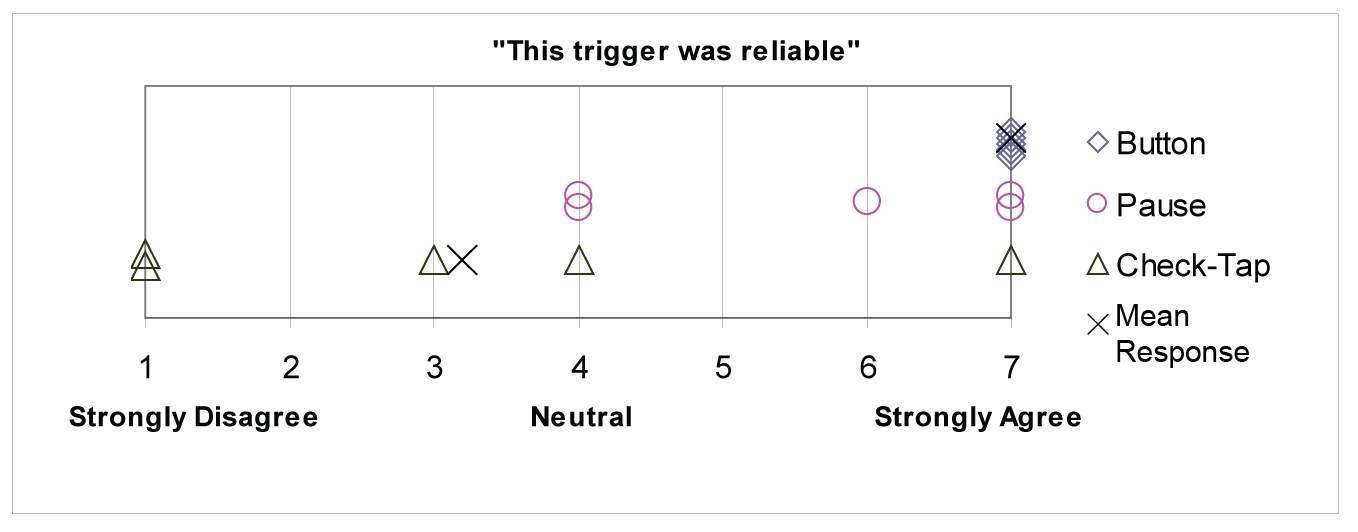
\includegraphics[width=1.0\linewidth]{buttonReliable-bigger.png}
  \caption{\label{fig:buttonReliabilityChart}
           Individual user respose to recognition trigger
           reliability. ``X''s show mean values.}
\end{figure}

%% Quotes not used:
%% Another user commented with frustration that the Gesture
%%Trigger was "very unreliable" and that the Button Trigger was
%%(desirably) much more "consistent."  

\subsection{Separation/Annotation Tools}

\begin{table}
  \centering
	\begin{tabular}{|p{.45\linewidth}|c||c|}
	\hline 
  Question 																									& Color Tool & Lasso Tool \\
  \hline
  This annotation tool was convenient to use.								& $6.2\pm0.4$ & $3.2\pm1.3$  \\
  \hline
  I felt comfortable using this annotation tool.						& $6.6\pm0.5$ & $5.0\pm1.0$  \\
  \hline
  This annotation tool was reliable.												& $6.0\pm1.0$ & $4.0\pm1.4$  \\
  \hline
  This annotation tool was efficient.												& $6.5\pm0.5$ & $3.4\pm1.1$  \\
  \hline
  My experience using this annotation tool was satisfying.	& $6.2\pm0.8$ & $3.4\pm1.1$  \\
  \hline
	\end{tabular}
	\caption{Questionnaire results for Annotation Tools.}
	\label{tab:TableBAnnotationData}
\end{table}


Table~\ref{tab:TableBAnnotationData} summarizes user response to
survey questions about separation techniques.  Users unanimously
preferred the pre-separation (color) tool to the post-separation
(lasso) tool, and all users found the pre-separation tool more
satisfying to use than the post-separation tool (Figure
\ref{fig:annotationSatisfaction}).  Many modal interfaces
traditionally suffer from the problem that users often forget to
toggle to the appropriate mode before performing a task.  However, in
our study, only one of five users forgot to toggle the Color Tool into
annotation mode before writing notes; furthermore, this user corrected
her mistake immediately.

Two participants commented that the lasso tool constrained the way
they could create their diagrams.  One user described that
the color tool "required less planning about where and when to write
so as not to screw up [the] lasso[] [gesture]."  Another user
commented that she "like[d] the [Color Tool's] ability to draw
annotations wherever" she wanted and that the color tool "saves [the]
inefficient circling motion" of the lasso tool.  

One issue that may have influeced users responses to the separation
mechanism is that the lasso tool required two check-tap gestures while
the color tool required only one.  The unreliability of the check-tap
gesture influences user reactions to the annotation tools,
nevertheless, users responded more negatively to the burden of
circling the symbols and the physical segregating of notes and
schematic strokes than to executing the gesture.  One user even modified 
her questionaire to express her preferences for Annotation Tools that 
hypothetically used the button trigger rather than check-tap; this user 
still preferred the color tool.

%I don't think you need this part.  
% Two users noted that
%both annotation tools suffered from the lack of reliability of the
%Check-Tap Gesture.  Operation of the Lasso Tool requires execution of
%two Check-Tap gestures while operation of the Color Tool requires only
%one.  Though the reliability issue surrounding the Check-Tap gesture
%colors user reactions to the annotation tools, the fact remains that
%the Lasso Tool requires more effort in circling symbols and the
%physical segregating of notes and schematic strokes.  Clearly the
%potential for confusion over the multi-modal nature of our
%Pre-separation tool imposed a minimal and acceptable burden on users.

\begin{figure}[tb]
  \centering
  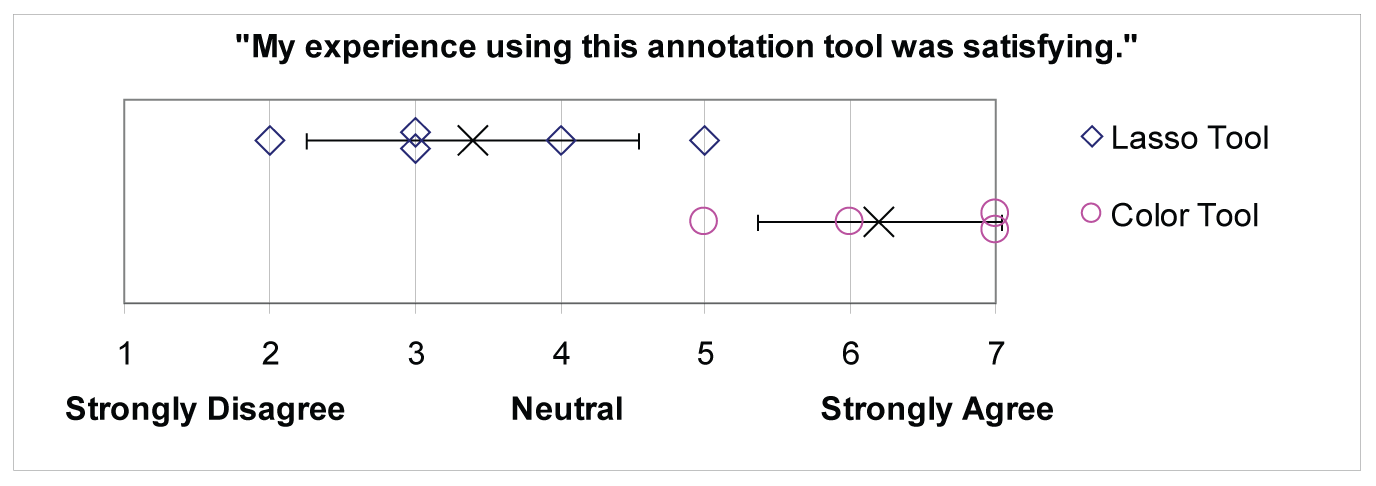
\includegraphics[width=1.0\linewidth]{annotationSatisfying.png}
  \caption{\label{fig:annotationSatisfaction} Individual user
           responses to sketch separation method satisfaction.}
           
\end{figure}



\subsection{Feedback Mechanisms}

\begin{table}
  \centering
	\begin{tabular}{|p{.45\linewidth}|c||c|}
	\hline 
  Question 																									& Color & Text-Label \\
  \hline
  This feedback mechanism produced understandable results.	& $7.0\pm0.0$ & $6.5\pm0.5$  \\
  \hline
  I would feel comfortable submitting the result on my screen as a diagram for my homework.
  																													& $6.5\pm0.5$ & $5.0\pm1.9$  \\
  \hline
  This feedback helps me work efficiently.									& $6.3\pm1.2$ & $5.1\pm1.6$  \\
  \hline
  The feedback was distracting.															& $1.1\pm0.4$ & $3.1\pm2.4$  \\
  \hline
  The feedback was confusing.																& $1.3\pm0.5$ & $2.1\pm1.6$  \\
  \hline
  My experience using with this feedback mechanism was satisfying.
  																													& $6.5\pm0.5$ & $5.5\pm1.9$  \\
  \hline
	\end{tabular}
	\caption{Questionnaire results for Feedback Mechanisms.}
	\label{tab:TableC1FeedbackData}
\end{table}


Table~\ref{tab:TableC1FeedbackData} summarizes user survey responses
to feedback mechanisms.  Users unanimously liked color feedback, and
most users preferred color feedback to text-label feedback.  Users
found text feedback distracting (Figure
\ref{fig:feedbackDistracting}), and that it added an unnecessary
mental burden to the design process.  One user commented that "The
text gets very cluttered [and] covers up the [sketch's] points of
interest quickly," thus interrupting his ability to reason about the
diagram.  Another user commented that text labels "can get a little
distracting with four or five [instances] of the same gate" and finds
the color feedback "more elegant" and "less redundant."  While our
specific text placement may have influenced user perception of the
text labeling feedback mechanism (i.e., sometimes the text obscured
part of the sketch), automatic text placement is a difficult problem,
and any automatic text placement method will likely obscure some
portion of the user's sketch.

%% Furthermore, the cluttering issue surrounding Text Feedback suggests
%% users might have expressed equal disdain for feedback through stroke
%% substitution (e.g., through Symbol Replacement).  We did not develop
%% and test Symbol Replacement due to the lack of common interest in this
%% feedback during our paper prototype study; furthermore, Symbol
%% Replacement Feedback presented technical challenges that would make
%% development impractical for our project's timeframe.  Originally we
%% had considered two possible implementations for Symbol Replacement:
%% one implementation that faintly overlays symbols over a sketch and one
%% implementation that completely erases and replaces user strokes with
%% symbols.  The overlay implementation would have entailed even more
%% sketch obfuscation than that of text labels, thus we anticipate that
%% users would still have preferred Color Feedback.  Moreover, the
%% obfuscation issue that our users raise negates an implementation that
%% entails complete stroke replacement.  Complete stroke replacement
%% would necessarily destroy user strokes and completely prevent users
%% from comparing recognition result labels (e.g., B\'{e}zier Curve
%% symbols) to raw ink symbols.

Despite the distracting nature of text feedback, many users still
appreciated the ease of reading text labels.  One user commented that
she "like[d] both" methods of feedback and found that "a button to go
back and forth [between feedback mechanisms] would be nice."  The
informal responses of three other participants corroborate the
usefulness of a feature for toggling text labels.  On the other hand,
one user specifically opined against such a toggle feature because he
found the obfuscation of text feedback made this type of feedback
impractical for use.  However, the (sole) user who ranked text
feedback as the most desirable (as noted in Table C2) asserted that
the text labels did not bother him and that "It's easier to
distinguish gates by their name rather than [through the use of]
different colors."  During the Color Feedback tests, each of the six
participants immediately inspected recognition results through
hovering her or his stylus over individual gates in order verify the
labels of symbols.  Though no participant claimed that the necessity
of learning the mapping of colors to labels presented an unacceptable
obstacle to using the system, cognizance of this color mapping alone
does not fully support the task of interpreting feedback.

\begin{figure}[tb]
  \centering
  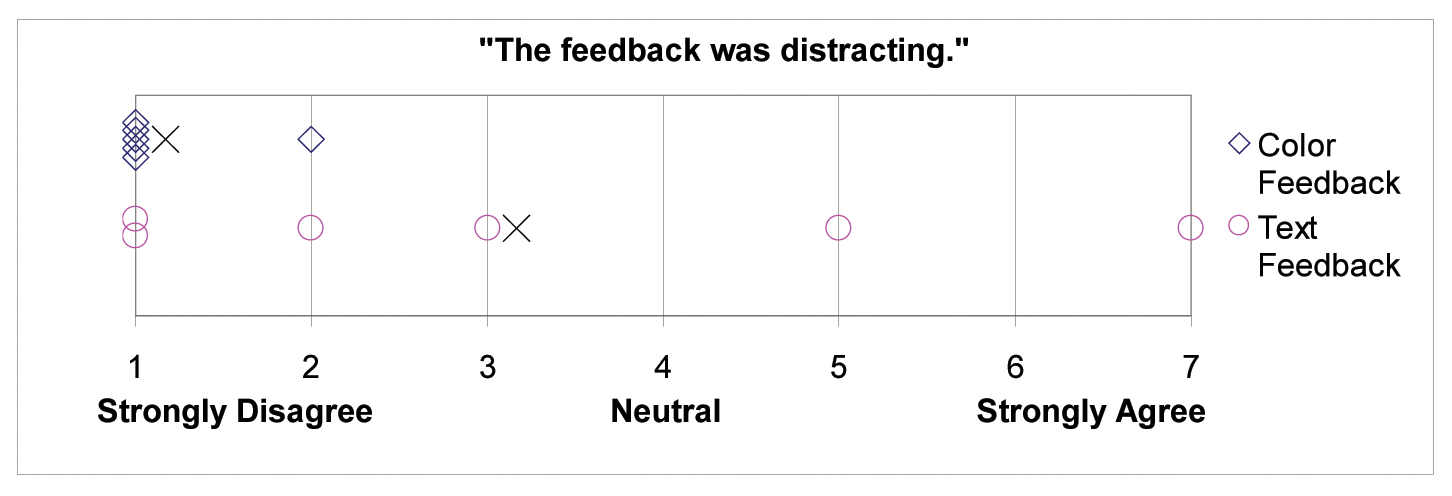
\includegraphics[width=1.0\linewidth]{feedbackDistracting.png}
  \caption{\label{fig:feedbackDistracting}
           Individual user responses to feedback distraction level}
\end{figure}

%% Unused text:
%In contrast, this user found the "hover"
%feature of Color Feedback "less distracting."  The text labels'
%obfuscation of the sketch causes user distress.  In response to the
%issue of obfuscation, one user exclaimed that he "[couldn't] tell what
%gate [he] drew [when he drew] small gates."  Obfuscation taints the
%Text Feedback's aesthetic.  

\subsection{Error Types}


\begin{table}
  \centering
	\begin{tabular}{|p{.35\linewidth}|c||c||c|}
	\hline 
  Question 																									& Mislabel & Omission & Group \\
  \hline
  Detecting errors was difficult. 													& $2.3\pm1.0$ & $2.6\pm1.9$ & $3.5\pm1.2$ \\
  \hline
  These errors frustrated me. 															& $4.5\pm2.2$ & $4.0\pm2.0$ & $4.1\pm1.3$ \\
  \hline
  Correcting errors was cumbersome. 												& $3.8\pm1.6$ & $2.8\pm1.5$ & $3.0\pm1.9$ \\
  \hline
  I attempted to understand why the system produced errors.	& $3.0\pm1.9$ & $3.3\pm1.6$ & $3.3\pm2.7$ \\
  \hline
  If I continued to encounter this type of error during further use of this application, I would change how I sketch.																																					& $3.0\pm2.1$ & $3.6\pm1.8$ & $4.8\pm1.7$ \\
  \hline
  These recognition errors confused me.											& $3.5\pm2.1$ & $3.0\pm1.9$ & $3.0\pm1.3$ \\
  \hline
	\end{tabular}
	\caption{Questionnaire results for error types.}
	\label{tab:TableDErrorData}
\end{table}


Users had diverse reactions to recognition errors.
Table~\ref{tab:TableDErrorData} summarizes user survey responses; the
survey results unfortunately do not illustrate any major trends.


%Figure \ref{fig:errorChangeSketch} indicates that users tended to be
%more willing to adapt their sketching styles in response to grouping
%errors.  Though three of six users expressed that they would be
%willing to adapt to the system in order to reduce errors, qualitative
%user reactions were not as consistent.

One reason our quantitative results show no strong trends may be due
to an unintended effect of the way we generated errors.  To keep error
rates consistent, the computer system automatically generated
ommission and false positive errors.  However, generating grouping
errors was too difficult to automate (it would require a deeper
understanding of the sketch in order to split and merge adjacent
groups), so the human user generated grouping errors.  Consequently,
false positives and omissions were often more surprising to users
(e.g. a wire classified as an AND gate) than grouping errors.  This
effect limits the direct comparison we can make between user response
to error type, but allows us to better understand the importance of
how users perceive errors based on how well they can understand them.

Our qualitative results suggest that user acceptance of the system is
related not only to absolute error rates but also to how well they
understand and trust the system's recognition.  Generally, our users
were initially happy to correct any type of recognition error, but
quickly became frustated when they could not understand why errors
occurred.  Two users specifically explained that his acceptance of the
system would depend not on the error rate as much as on the
predictability of errors.  Another user remarked that he would not be
willing to accept a system with the error rate exhibited unless errors
were more predictable and helped him adapt his drawing style to avoid
them.  This user also found false negatives the most confusing because
these errors failed to inform him about "what to move away from"
(i.e., how to change his sketching style to reduce error).  On the
other hand, another user preferred false negatives because it made him
trust the system more when it did recognize his strokes.

%% User frustration with errors stems from the inability to establish a
%% reliable and practical mental model of errors.  Generally, users are
%% initially happy to correct any type of recognition error.  Repeated,
%% frustrating errors will inspire users to commit modest yet pragmatic
%% mental effort to understanding errors.  If users fail to learn to
%% predict errors, then frustration will lead them to distrust and reject
%% the system.  Indeed, we found that acceptance of this tool hinged on
%% frustration with, and the predictability of, errors.  Two users
%% remarked that they would accept the current error rate as-is.  Another
%% user also expressed acceptance of the current error rate and remarked
%% that the time required to correct recognition errors with our system
%% was comparable to the time she spent correcting errors while using the
%% WIMP applications her coursework requires.  One user specifically
%% rejected our interface based upon the exhibited error rate and
%% specified that he would only find one recognition error per circuit
%% schematic acceptable; however, this user responded that he was only
%% "kind of" able to predict errors.  The remaining two users both
%% explained that their acceptance of the system depended heavily on the
%% predictability of errors.  One user explained that he would accept the
%% system only if he could reasonably "adapt to" it and that he wanted
%% system errors to help inform his drawing style.  The other emphasized
%% the impact that error rate had on his trust of the system.  This user
%% explicated that he would trade a higher omission error rate for lower
%% grouping and mislabel error rates.  He explained that "if [the system]
%% says 'I don't know what [a sketched symbol] is' then that's a good
%% thing"; a tendency to omit labels rather than incorrectly assign
%% labels helps make the system "safer" to use.  The predictably and
%% acceptance of errors is crucial to an interface's trustworthiness.



We also found that users created dramatically different mental models
of errors.  Two users considered themselves responsible for grouping
errors; one user remarked that grouping errors were related to her
sketching style.  Two users blamed the system for mislabel and
omission errors.  One of these users remarked that mislabel and
omission errors seemed "out of context," or unpredictable.  Two users
specifically remarked that they did not try to form a mental model of
errors.  

\textit{Not sure if this is right!} Qualitative user responses related
to frustration with errors exhibited a strong trend.  Four out of six
users responded that omission errors were the easiest to perceive;
users likely find that the lack of a label is easier to detect than an
incorrect label.  Furthermore, four out of six users remarked that the
grouping error was the most confusing type of error, despite the fact
that these errors were human-generated.


%% Three users indicated that they would be
%% inclined to change their sketching styles in order to deal with
%% grouping errors (see Figure \ref{fig:errorChangeSketch}).  One user
%% who responded positively to this survey question (giving a rating of
%% 7/7) also found grouping errors the most confusing; however, this user
%% explained her reaction as a result of the fact that grouping errors
%% were her first exposure to errors.  Two other users who responded
%% positively to the survey question (both giving a rating of 6/7)
%% remarked that they did not attempt to form a mental model of errors.
%% Therefore, users who found grouping errors the most confusing gave
%% survey responses that they were the least likely to change their
%% sketching styles in reaction to grouping errors. \textit{This needs
%% more explanation--it's a little confusing}

%% % plot for survey question "I would change my sketching style of these errors continued..."
%% \begin{figure}[tb]
%%   \centering
%%   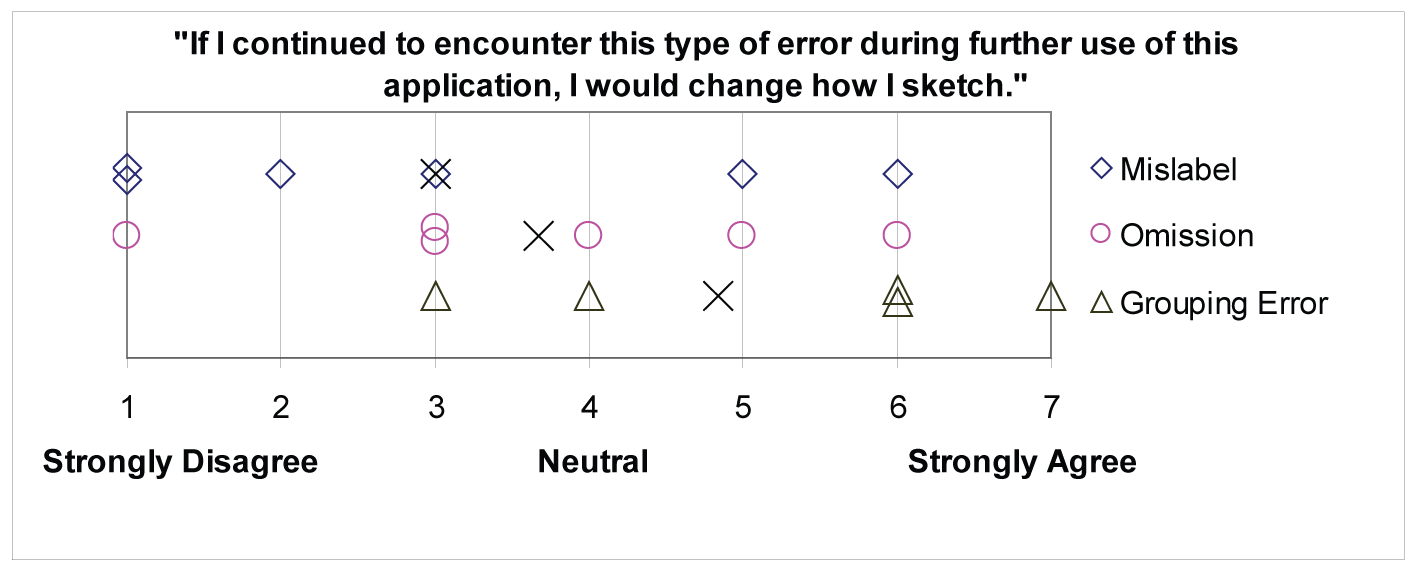
\includegraphics[width=1.0\linewidth]{errorChangeSketch.png}
%%   \caption{\label{fig:errorChangeSketch}
%%            Individual user responses to whether or not they
%%            would change their sketching style}
%% \end{figure}

%User reactions to other types of errors corroborate a trend that
%confusion leads to rejection of the system.  Expressing angst over the
%unpredictability of the randomly generated mislabel errors, one user
%asserted that "[he] would probably not change [his drawing] techniques
%to match the tool, [he'd] just not use the tool."  This user also
%specifically explained that his acceptance of the system would depend
%on the predictability of errors.  Another user expressed similar angst
%with mislabel errors and commented that they were   ; this user was willing to adapt his style to the
%system but explains that the lack of a correct or incorrect label
%fails to enable him to change his style.  

Finally, the error correction process also impacted user reactions to
the system.  Three users remarked that more effective error correction
mechanisms would help ameliorate the frustration of dealing with
errors.  Though most users were comfortable using the erase gesture to
erase and redraw incorrectly recognized symbols, one user found the
erase gesture hard to control because of the size of the stylus'
eraser.  Another user requested a selection tool for erasing large
amounts of ink.

%%  and the final user requested support for debugging
%% circuit connections.  The remaining user specifically requested a 'netlist'
%% feature that would allow a user to visually highlight and debug
%% connections between symbols.  This 'netlist' feature would both aid in
%% the verification of a circuit design and help users detect grouping
%% errors.
  



%-------------------------------------------------------------------------
%% \section{Error Analysis}
%% \textit{This stuff should be integrated into the text above, rather
%%   than presented as one big disclaimer at the end.  I've tried to do
%%   this and commented out the stuff that I think is integrated (see
%%   comments in the latex source).  Are
%%   any of our results statistically significant?}

% I think I covered most of this paragraph in the first part of the
% results section. 
%% Most of our survey data fails to provide a statistically significant
%% foundation for the identification of solid trends in user preferences.
%% Furthermore, in some cases our users presented conflicting viewpoints
%% in response to qualitative questions.  Most traditional evaulation
%% techniques and questionaires measure the overall performance of an
%% application with respect to well-established axes of macroscopic
%% system characteristics (I have no reference for this, its just an
%% observation).  However, our study breaks new ground in attempting to
%% inform system design through the juxtaposition of contrasting
%% interface elements.  Through our evaluation measures and experimental
%% methodology, we have more effectively illuminated apposite axes of
%% interface element characteristics than measured against an existing
%% metric.

% This paragraph is covered with the presentation of results.
%% The unreliability of the Check-Tap gesture confounded user reactions
%% to Recognition Triggers and Annotation Tools.  This confounding
%% prevents conclusively determining one Recognition Trigger or one
%% Annotation Tool as maximally efficacious.  However, our inquiry
%% illuminates how the efficacy of Recognition Triggers and Annotation
%% Tools are directly related to how well these interface elements
%% support efficient work.  Despite the exceptionally high gesture error
%% rate observed, the emphasis of user responses on the importance of
%% reliability suggest that gestures may make inherently impractical
%% Recognition Triggers.  Furthermore, qualitative user feedback
%% comparing the Color and Lasso Annotation Tools emphasizes users'
%% preference for efficiency and simplicity.  Users see convience and
%% novelty as secondary characteristics.

% Incorporated above.
%The implementation of the Text-Label Feedback partially counfounded
%legibility of recognition results.  Two users complained that text
%labels often made recognition results illegible because labels would
%completley obfuscate small gates.  Despite this quirk, any labeling
%method will entail some amount of obfuscation of the sketch.  User
%responses emphasize the importance of the minimization of distracting
%aspects of feedback, therefore any label-based Feedback Mechanism may
%fail to maximize the efficacy of feedback.

%% \textit{Paul: Explain this in the study design and get rid of the text
%%   here.  Justify why it makes sense to allow users to choose their
%%   preferred feedback mechanism (i.e., makes them more likely to spot
%%   errors because they are using the feedback they prefer) instead of
%%   saying it confounds results.}
%% Furthermore, our study of Feedback Mechanisms confounded our study of
%% Error Types.  We did not balance the Feedback Mechanisms used across
%% Error Type study sessions and instead allowed users to choose which
%% method of feedback to use.  Most users preferred and used Color
%% Feedback; the experimenter also invited users to complete part of the
%% Error Type study using the alternate Feedback Mechanism so that users
%% could compare the two.  Three users commented that the visual contrast
%% between symbols provided by Color Feedback helped them spot errors.
%% No user mentioned that either feedback mechanism prevented them from
%% finding errors.  Our study's results emphasize that users desire high
%% visibility of errors.


%% \textit{This text really needs to be incorporated into the dicsussion
%%   of error perception above. I will take care of this.} 

 
%-------------------------------------------------------------------------
\section{Discussion}
The results of our study inform the design of educational sketch
recognition systems.  Here we summarize the major implications for
both user interface and recognition engine developers.

\textbf{Recognition triggers should be user-triggered, efficient and
reliable.} Our study illuminates that, with respect to our tasks, user
prefer reliability as much as they do convenience.  Gestures and
system activated recognition may be an option, but should not be the
only option.  

\textbf{The interface should provide users with a way to separate
recognized from unrecognized strokes as they draw.}  Users desire
efficiency and are willing to put in small amouts of effort while they
work to avoid larger amounts of effort later in the process.  Our
study participants preferred our pre-separation for its relatively low
mental and physical overhead.

\textbf{Recognition feedback should transform users strokes as little
as possible.} Stroke color effectively provides contrast between
recognition labels with minimal stroke transformation.  More dramatic
transformation of user strokes should only occur upon user request.

\textbf{Users are willing to correct errors after they are done
drawing.}  Our users were willing to correct errors, treating it as a
game or a necessary evil.  Consistent with previous work in
recognition-based user interfaces, they do error correction all in one
batch and tend not want to disturb their design process with
on-the-fly correction.  

\textbf{Errors must be predictable and/or understandable} Automatic
recognition engines potentially can make non-sensical errors.
Recognition engines that incorporate adjustable confidence levels may
help user interface designers strike an optimal balance between false
positives and false negatives.  A recognition engine that could
describe precisely why a given interpretation was missed could also
users' modify their drawing styles to raise recognition rates.  


%% \begin{itemize}
%% \item \textbf{To interface developers} triggers must be efficient and
%% reliable.  system-activated recognition can be an option, but should
%% not be the only option
%% \item \textbf{To interface developers} efficiency is what users want.
%% annotation/seperation tools should either work passively
%% (e.g. notes/sketch panel) or require minimal effort (color tool).
%% \item \textbf{To interface developers} least distracting feedback is
%% best=>feedback that involves minimal transformation of user strokes is
%% best.  text labels or symbol replacement is something that should
%% occur only upon user request.
%% \item \textbf{To interface developers} users treat error correction as
%% a game or a necessary evil.  they do error correction all in one batch
%% and tend not want to disturb their design process with on-the-fly
%% correction or feedback about errors in their sketch.  Minimization of
%% the error rate and enhacement of the visibility of errors are possible
%% ways to alleviate frustration.
%% \item \textbf{To recognition engine developers} The predictability of
%% errors minimizes frustration and reduces the chance of system
%% rejection.  It is possible that only labeling symbols that have high
%% confidence might be an effective way to ensure predictability.
%% Trainable recognition could also help.

%\item \textbf{To those who educate users} User emphasis on
%predictibility suggests that users desire well-defined interaction
%paradigms.  this might be taking things a bit too far...
%\item \textbf{To those who educate users} Our users were most excited
%to use a tablet because it's a tablet.  We cannot conclude that
%tablets afford higher efficiency, but we can conclude that tablets
%arouse the internal motivation of students and make them more
%efficient workers.  again, this might be taking things a bit too
%far...
%\end{itemize}

%-------------------------------------------------------------------------
\section{Conclusion}
We have presented an initial comparison of interface elements for
free-sketch recognition systems that both guides user interface
development and suggests other important questions to explore.  Future
studies should examine reaction to error rate, type and correction
mechanism in more detail.  In addition, while some of our users
expressed a moderate willingness to modify their drawing style to
reduce recognition error, more work is needed to determine the optimal
balance between a gesture-based and free-sketch interface.

Perhaps the most important outcome of our user study was the excitment
users showed for a sketch-based user interface to replace the
cumbersome interface they currently use.  The major advantage they
perceived in a sketch-based interface is the lower cognitive load in
entering their circuits and the expressed a willingness to cope with
and correct the recognition errors inherent with such a system.



%-------------------------------------------------------------------------
\section{Acknowledgments}
We would like to thank our study participants and our Wizard, Kris
Karr.  We would also like to thank Susan Matonosi and Deb Mashek for
helpful feedback on our study design.  This work is supported in part
by an NSF CAREER award (IIS-0546809).


%-------------------------------------------------------------------------




%
% NOTES
%

% User A = Roz 
% User B = Pokey
% User C = Elton
% User D = Jason
% User E = Mackenzie
% User F = Thomas
% User G = Heather
% User H = Matt W
% User I = Max P



%max
%one user 4 sec pause is too long
%one user 10-15 check taps before a go
%more than 10 gates, would trigger more than once, but can get everything in his head as it is
%5-10 checks before it worked for annotation mech
%says it is more natural to have notes in sketch
%no tablet in e85, but yes tablet experience

%pokey yes tablet
%5 times check tap till worked
%10+ check taps in annotatio mech

%RB no tablet
%2/2 in tuturial, then 5 bad checktaps
%"I like the dot" the dot is emphatic
%errs-> "I always feel like I lose when it turns red"
%button has "all the benefits of the check-tap [trigger] but non of the bad stuff"
%five checktap failures in annotations

%MW e85 tutor, no tablet
%6 for 6 on checktap
%"marginal difference" but did prefer it cuz it was easier, liked manually doing checktap
%4 sec pause too long
%1/6 on color tool, 1/3 on lasso tool
%asso is "a little too much work"

%heather yes tablet
%check tap 3/4 during tutorials
%then 1/4 and 3/7, and then 7/10 for lasso



\bibliographystyle{eg-alpha}
\bibliography{UserStudyPaper-bibio}





\end{document}
